%----------------------------------------------------------
\def\notedate{2021.11.14}
\def\currentauthor{Муха В. (РК6-73Б)}
%----------------------------------------------------------
\notestatement{rndhpcedt}{Первичный обзор литературы}

%----------------------------------------------------------
\subsubsection{Известные алгоритмы поиска циклов в графах}

%Следующий материал является результатом анализа работы.

%\paragraph{Алгоритмы обхода}

Существует несколько групп алгоритмов поиска\cite{davidrajuh2016}:
\begin{enumerate}[label=\arabic*)]
    \item алгоритмы ``прохода'';\messnote{Очень общее и не стандартное название. Известны алгоритмы обхода ориентированных графов... притом разные. Прошу уточнить.}
    \item алгоритмы, основанные на использовании матриц смежности.
\end{enumerate}

Одним из представителей алгоритмов ``прохода'' является алгоритм depth-first-search (DFS). Сложность алгоритма $O(n^2)$ для одного прохода и $O(n^3)$ -- для всех проходов.\messnote{Что значит для всех проходов? Прошу уточнить.} Поэтому для ускорения алгоритма необходимо применение модификаций\cite{Mahdi2011}.\messnote{Каких? Немного подробнее.} 

Зададим граф $G(V, E)$, где $V$ -- это множество вержин графа $(a, g)$, а $E$ -- это множество рёбер графа $(ab, ad, ... , ge)$. Сам граф $G$ и его матрица смежности $A$ приведены ниже.\messnote{Всё же стоит набрать это.}

\begin{figure}[H]
	\centering
	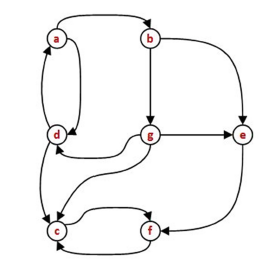
\includegraphics[width=0.3\textwidth]{ResearchNotes/rndhpc_not_edt_2021_11_14/adj_matrix.png}
	\caption{Граф и его матрица смежности} 
\end{figure}

Матрица смежности $A$ показывает в какие узлы можно ``попасть'' из текущего, а транспонированная матрица $A^T$ показывает из каких узлов возможно ``попасть'' в текущий.

%----------------------------------------------------------
\subsubsection{Поиск циклов в графах в т.ч. при помощи GPU}

Для того, чтобы определить циклы из двух шагов,\messnote{Непонятно. Термин ``цикл из шагов'' не является корректным.} нужно найти матрицу циклов $C$. Её можно найти, применив операцию \textsf{AND} над матрицами $A$ и $A^T$. \messnote{Указанную операцию стоит описать немного подробнее.}

\begin{equation}
    C = (A \wedge A^T)
\end{equation}

Таким образом, матрица $C$ будет содержать все циклы из двух шагов. Для определения циклов из большего количества шагов необходимо применить операцию повторно.

\begin{remark}
Поиск циклов в графе является NP-полной задачей\cite{YYY}, следовательно \textbf{не может} быть выполнен за полиномиальное время.\messnote{ОШИБКА !}
\end{remark}

В статье \cite{Mahdi2011} представлен подход, позволяющий ускорить процедуру поиска циклов с использованием \textsf{GPU}, описываемый алгоритмом \ref{algo.cycles.search}.\messnote{Алгоритм следует описать много подробнее. Все объекты следует обозначить. Комбинация? Новый массив? Циклы в потоках?}

\begin{algorithm}[H]% <-------- do not float, stay right [H]ERE!
\caption{Алгоритм XXXX поиска циклов в ориентированном графе}\label{algo.cycles.search}
\begin{algorithmic}[1]
	\State Определяем особенности вычислительной системы.
	\State Создаем новый массив узлов.
	\State Для каждого узла параллельно создаём комбинацию для проверки.
	\State При помощи алгоритма DFS находим циклы в каждом из потоков.
	\State Повторяем алгоритм, пока не будут обнаружены все циклы.
\end{algorithmic}
\end{algorithm}

%----------------------------------------------------------
% Атрибуты задачи
\noteattributes{}
%----------------------------------------------------------